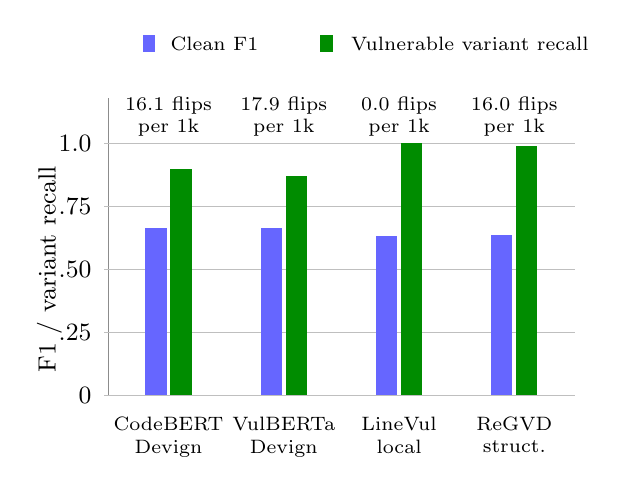
\begin{tikzpicture}[
  x=1.22cm,
  y=3.2cm,
  font=\small
]
\begin{scope}[shift={(0,-0.28)}]
\draw[black!45] (0,0) -- (4.85,0);
\draw[black!45] (0,0) -- (0,1.18);
\foreach \y/\label in {0/0,0.25/.25,0.5/.50,0.75/.75,1/1.0} {
  \draw[black!25] (-0.05,\y) -- (4.85,\y);
  \node[anchor=east] at (-0.08,\y) {\label};
}
\node[anchor=center, rotate=90] at (-0.62,0.50) {F1 / variant recall};

% CodeBERT-Devign local
\fill[blue!60] (0.38,0) rectangle (0.60,0.665);
\fill[green!55!black] (0.64,0) rectangle (0.86,0.896);
\node[anchor=north, align=center, font=\scriptsize] at (0.62,-0.05) {CodeBERT\\Devign};

% VulBERTa local
\fill[blue!60] (1.58,0) rectangle (1.80,0.663);
\fill[green!55!black] (1.84,0) rectangle (2.06,0.870);
\node[anchor=north, align=center, font=\scriptsize] at (1.82,-0.05) {VulBERTa\\Devign};

% LineVul local
\fill[blue!60] (2.78,0) rectangle (3.00,0.630);
\fill[green!55!black] (3.04,0) rectangle (3.26,1.000);
\node[anchor=north, align=center, font=\scriptsize] at (3.02,-0.05) {LineVul\\local};

% ReGVD structural local
\fill[blue!60] (3.98,0) rectangle (4.20,0.637);
\fill[green!55!black] (4.24,0) rectangle (4.46,0.988);
\node[anchor=north, align=center, font=\scriptsize] at (4.22,-0.05) {ReGVD\\struct.};

\node[align=center, font=\scriptsize, fill=white, inner sep=1pt] at (0.62,1.105) {16.1 flips\\per 1k};
\node[align=center, font=\scriptsize, fill=white, inner sep=1pt] at (1.82,1.105) {17.9 flips\\per 1k};
\node[align=center, font=\scriptsize, fill=white, inner sep=1pt] at (3.02,1.105) {0.0 flips\\per 1k};
\node[align=center, font=\scriptsize, fill=white, inner sep=1pt] at (4.22,1.105) {16.0 flips\\per 1k};
\end{scope}

\fill[blue!60] (0.35,1.08) rectangle (0.48,1.15);
\node[anchor=west, font=\scriptsize] at (0.54,1.115) {Clean F1};
\fill[green!55!black] (2.20,1.08) rectangle (2.33,1.15);
\node[anchor=west, font=\scriptsize] at (2.42,1.115) {Vulnerable variant recall};
\end{tikzpicture}
